\subsection{Problem setting}
\label{sec:setting}

Consider one round of scaled dot-product attention over $N$ agents, per batch
element, at head width $d$. Agent $i$ forms a query $q_i$; every agent
contributes a key and a value; self-attention is masked. Write
$s_i = q_i K^\top \in \mathbb{R}^N$ for the score vector and
$a_i = \mathrm{softmax}(s_i)$ for the attention weights, so that dense attention
computes $m_i = a_i V$. A top-$k$ variant keeps the $k$ largest entries of $a_i$
and renormalises over them.

The mechanism this paper analyses is the one that arises most naturally from
that description: form the complete score vector, then keep its $k$ largest
entries. We call such a rule \emph{score-then-select}, and the term is used in
its exact sense throughout. Every analytic claim below concerns that class, not
content-dependent selection in general, and Section~\ref{sec:ceiling} draws the
boundary.

Attention has two matrix products of equal size. One produces the pairwise
scores; the other aggregates the values. Sparsifying the retained set shrinks
the second, because only $k$ value rows are combined. It cannot shrink the
first, because the scores are what the selection reads. That observation is the
whole of Section~\ref{sec:ceiling}; the rest of this section makes it precise
and marks where it stops applying.

Top-$k$ attention admits three implementations of the identical function, and
the distinction between them is what separates an arithmetic saving from an
executed one.

\begin{description}
  \item[Masked top-$k$.] Compute $a_i$ in full, multiply by a $\{0,1\}$ mask,
    renormalise, and evaluate $m_i = \tilde{a}_i V$ with $\tilde{a}_i$ still
    dense in memory. The discarded entries are materialised as zeros and
    multiplied, so the executed aggregation count is unchanged from dense while
    selection, masking and renormalisation are added on top.
  \item[Gathered top-$k$.] Take the top-$k$ of the raw scores, softmax over
    those $k$ values, gather the corresponding value rows into a $(B,N,k,d)$
    tensor, and contract $(B\!\cdot\!N,1,k)\times(B\!\cdot\!N,k,d)$. No zeros
    are materialised and the aggregation genuinely shrinks.
  \item[Fused top-$k$.] Compute the same function in a single kernel, holding
    the score row in registers, selecting within them, and accumulating the
    weighted values without writing a score matrix, an index tensor or a
    gathered value tensor to memory. Section~\ref{sec:fused} reports one.
\end{description}

\begin{figure}[t]
\centering
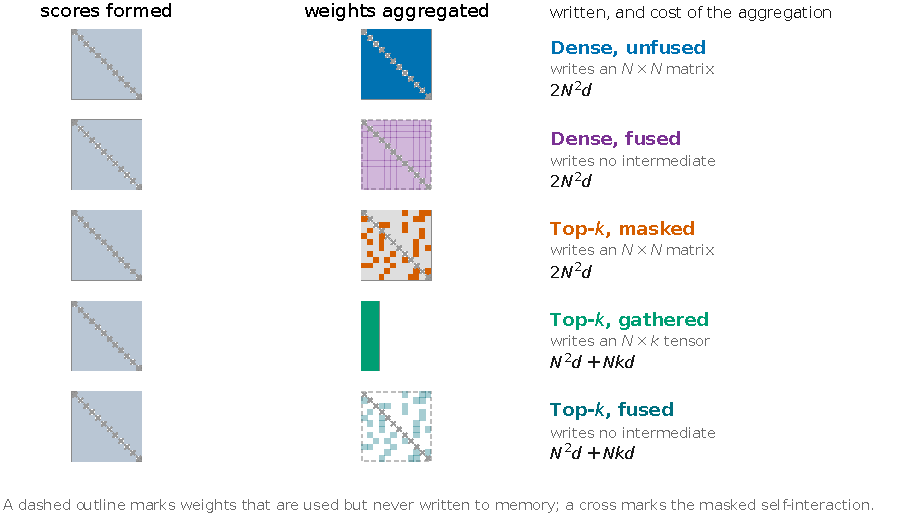
\includegraphics[width=\linewidth]{figures/fig1_taxonomy.pdf}
\caption{Two implementations of dense attention and three of top-$k$ attention,
computing two functions in five ways. All five evaluate every pairwise score,
because a score-then-select rule must form the complete score vector before it
can rank it. They differ in what reaches memory and in how much arithmetic the
aggregation performs, and only the gathered and fused top-$k$ variants execute
the saving that motivates sparsification at all. The fused row stands for the
kernels that compact the retained set; the threshold kernel of
Section~\ref{sec:fused} is fused in the same sense but keeps the dense
aggregation, so its cost is that of the masked row.}
\label{fig:taxonomy}
\end{figure}

Gathered and masked top-$k$ compute the same function
(Figure~\ref{fig:taxonomy}). Softmax is monotone within a row, so the top-$k$
weights are the top-$k$ scores, and a softmax over just those $k$ scores equals
the dense softmax restricted to them and renormalised; the two agree to
$<10^{-10}$ in \texttt{float64} (Appendix~\ref{app:verification}). The
operation-count argument is about the gathered variant. Timing the masked
variant measures an implementation artifact, and timing either against unfused
dense alone ignores what a production kernel costs, so we report all
implementations against both dense baselines throughout.

\subsection{An operation-count ceiling}
\label{sec:ceiling}

Analytic counts are multiply--accumulates. Under the convention that a
multiply--add is two floating-point operations every term doubles and every
ratio is unchanged, so the ceiling is the same number either way; we write MACs
where the count is analytic and FLOPs only where a counter attached to the
running program produced the figure. Counting the two matrix products that
constitute attention, and excluding the shared input and output projections:
\begin{equation}
C_{\text{scores}} = N^2 d, \quad C_{\text{agg}} = N^2 d, \quad
C_{\text{dense}} = 2N^2 d, \qquad
C_{\text{top-}k} = \underbrace{N^2 d}_{\text{all scores}} +
\underbrace{Nkd}_{\text{aggregate }k}.
\end{equation}

\begin{proposition}[Score-then-select ceiling]
\label{prop:ceiling}
Let the retained set be fixed by a score-then-select rule, one whose kept
indices are determined only after the complete score vector of each query has
been formed. Then
\begin{equation}
\frac{C_{\text{dense}}}{C_{\text{top-}k}}
= \frac{2N^2 d}{N^2 d + Nkd} = \frac{2N}{N+k} < 2
\qquad \text{for all } k \ge 1,
\end{equation}
with supremum $2$ approached only as $k/N \to 0$. Within this class, no choice
of $k$ or $N$ yields more than a twofold reduction in attention MACs.
\end{proposition}

\begin{proof}
$C_{\text{top-}k} > N^2 d = \tfrac12 C_{\text{dense}}$ for every $k \ge 1$ since
$Nkd > 0$, so the ratio is below $2$. It is decreasing in $k$, hence largest at
$k = 1$, and approaches $2$ from below as $k/N \to 0$.
\end{proof}

The familiar figure $1 - k/(N-1)$ describes the value-aggregation term alone.
Read as \emph{the} saving it overstates the achievable reduction by a factor
approaching two, before any question of whether the reduction is realised in
time.

We use $N^2 d$ rather than $N(N{-}1)d$ because it is the count the
implementations execute: self-masking writes $-\infty$ into the diagonal of a
full $N \times N$ score matrix and does not skip work. Counting the diagonal
exactly gives $2(N{-}1)/\bigl((N{-}1)+k\bigr)$, which is strictly smaller for
every $1 \le k \le N-1$, so the proposition is a valid upper bound under either
convention.

The ceiling is a statement about the forward pass, and training moves it. Exact
selection is piecewise constant in the scores, so gradients reach only the
retained entries: of the four products in dense attention's backward pass
(the gradients with respect to values, weights, queries and keys, each
$N^2 d$), a gathered top-$k$ backward executes each over the $Nk$ retained pairs
alone, given the indices recorded in the forward pass. Counting both passes,
without recomputation,
\begin{equation}
\frac{C^{\text{f+b}}_{\text{dense}}}{C^{\text{f+b}}_{\text{top-}k}}
= \frac{6N^2 d}{N^2 d + 5Nkd} = \frac{6N}{N+5k} < 6,
\end{equation}
so in training at most five sixths of attention's arithmetic is removable,
against half in inference. The asymmetry is visible in the measurements of
Section~\ref{sec:backward}, where the gathered path's backward is cheap relative
to its forward.

Six assumptions support the statement, of which only the second is essential.
\textbf{(A1) Single round}: with $R$ rounds both terms scale by $R$ and the
ratio is unchanged. \textbf{(A2) Full-score selection}: the retained set is
determined only after the complete candidate score vector has been computed, so
all $N$ scores must be formed. \textbf{(A3) Per head}: with $H$ heads of width
$d/H$ both terms scale identically. \textbf{(A4) Projections excluded}:
including the shared $qkv$ and output projections moves the ratio strictly
closer to $1$, so the bound remains valid. \textbf{(A5) Selection cost
excluded}: counting the top-$k$ operation itself can only decrease the ratio,
and Section~\ref{sec:stages} shows the term is large in practice.
\textbf{(A6) Equal key and value widths}: with key width $d_k$ and value width
$d_v$ the two products cost $N^2 d_k$ and $N^2 d_v$, and the ceiling is
$1 + d_v/d_k$, which is $2$ in the equal-width attention used throughout.

A2 concerns \emph{when} the retained set is fixed, not whether the rule depends
on the data. Mechanisms that are content-dependent but not score-then-select lie
outside the class and are unconstrained by Proposition~\ref{prop:ceiling}: exact
or approximate nearest-neighbour retrieval, clustering and routing, indexing and
hashing can all identify candidates without materialising the complete pairwise
score matrix. Routing Transformer's online $k$-means routing
\citep{roy2021routing} and Reformer's locality-sensitive hash
\citep{kitaev2020reformer} are content-dependent in every ordinary sense and
still evaluate scores only for candidate pairs; a hierarchical rule that ranks
compressed blocks and then scores only the selected ones \citep{yuan2025nsa} is
likewise outside A2. What such rules pay instead is a selector cost, and the
next proposition charges them for it.

\subsection{Selection before scoring}
\label{sec:escape}

\begin{proposition}[Escape]
\label{prop:escape}
Suppose the kept set is determined \emph{without} forming the complete score
vector --- structurally, or by a retrieval, routing, clustering, indexing or
hashing rule --- at total selector cost $C_{\mathrm{sel}}(N,k,d)$, and that
attention scores are then evaluated only for the $Nk$ retained pairs. Then
\begin{equation}
C_{\mathrm{pre}} = 2Nkd + C_{\mathrm{sel}},
\qquad
\frac{C_{\text{dense}}}{C_{\mathrm{pre}}}
  = \frac{2N^2 d}{2Nkd + C_{\mathrm{sel}}}.
\end{equation}
\emph{(i)} If $C_{\mathrm{sel}} = o(Nkd)$ --- in particular for a fixed or
precomputed pattern, where $C_{\mathrm{sel}} \approx 0$; note that an
$O(N \log N)$ selector does \emph{not} qualify, since
$N\log N / (Nkd) = \log N/(kd) \not\to 0$ --- the ratio is
asymptotic to $N/k$, that is
$\bigl(C_{\text{dense}}/C_{\mathrm{pre}}\bigr)\big/(N/k) \to 1$. Exact equality
with $N/k$ holds only when $C_{\mathrm{sel}} = 0$; for every
$C_{\mathrm{sel}} > 0$ the ratio is strictly smaller. \emph{(ii)} If only
$C_{\mathrm{sel}} = o(N^2 d)$ and $k/N \to 0$, the ratio diverges, and in
particular is not bounded by $2$, though it does not in general grow at the
rate $N/k$.
\end{proposition}

\begin{proof}
Both statements read off the displayed ratio. For (i),
$2Nkd + C_{\mathrm{sel}} = 2Nkd\,(1+o(1))$, so
$C_{\text{dense}}/C_{\mathrm{pre}} = (N/k)\,(1+o(1))^{-1}$, whose quotient with
$N/k$ tends to $1$; substituting $C_{\mathrm{sel}} = 0$ gives
$2N^2 d/2Nkd = N/k$ exactly, and any $C_{\mathrm{sel}} > 0$ strictly enlarges
the denominator. For (ii), if $k/N \to 0$ then $2Nkd = o(N^2 d)$, so the whole
denominator is $o(N^2 d)$ and the ratio diverges.
\end{proof}

Proposition~\ref{prop:ceiling} is the limiting case of this accounting. A
score-then-select rule must form the full score matrix before it can rank it,
and in doing so it has already evaluated the scores of the $Nk$ retained pairs,
which the displayed form charges again inside $2Nkd$. Written in that form its
selector cost is therefore at least the scores of the discarded pairs,
$C_{\mathrm{sel}} \ge N^2 d - Nkd$, and this is a lower bound and not an
estimate: the ranking itself is uncounted, and counting it enlarges
$C_{\mathrm{sel}}$ and shrinks the ratio further. Substituting the bound gives
$2N^2d/(N^2d + Nkd)$, which is Proposition~\ref{prop:ceiling}; any real
implementation sits below it. Reading the two propositions as one statement
places any peer-selection mechanism on a single axis, the cost of deciding what
to keep, and the position on that axis determines what the mechanism can save.

\begin{corollary}[What a selector costs, and what it can therefore buy]
\label{cor:taxonomy}
Count $C_{\mathrm{sel}}$ in multiply--accumulate equivalents, one comparison,
integer operation or distance term being one unit. Fix $k$ and $d$ and let
$N \to \infty$ in $S = 2N^2d/(2Nkd + C_{\mathrm{sel}})$.
\emph{(a) Full-score selection}, $C_{\mathrm{sel}} \ge N^2 d - Nkd$: $S < 2$.
\emph{(b) All-pairs selection in a cheaper feature dimension $p \ll d$},
$C_{\mathrm{sel}} = \gamma N^2 p$: $S \to 2d/(\gamma p)$, a constant that does
not grow with $N$ and does not improve with $k$.
\emph{(c) Sub-quadratic selection}, $C_{\mathrm{sel}} = \Theta(N \log N)$:
$S = \Theta\bigl(Nd/\log N\bigr)$, which diverges, but is a vanishing fraction
of $N/k$.
\emph{(d) Fixed or precomputed patterns}, $C_{\mathrm{sel}} = o(Nkd)$ and in
particular $C_{\mathrm{sel}} \approx 0$: $S \sim N/k$. A selector with
$C_{\mathrm{sel}} = cNkd$ for a constant $c > 0$ gives $S \to 2N/((2+c)k)$,
which is $\Theta(N/k)$ but not asymptotic to it.
\end{corollary}

The asymptotic classes do not depend on the unit convention; the constants in
the closed forms below do.

\begin{proof}
Each case substitutes its $C_{\mathrm{sel}}$ into the denominator. In (b) the
$\gamma N^2 p$ term dominates $2Nkd$, giving $S \to 2N^2d/(\gamma N^2 p)$. In
(c) the $\Theta(N\log N)$ term likewise dominates $2Nkd$, giving
$S = \Theta(N^2 d / (N \log N))$; the quotient $S/(N/k) = \Theta(kd/\log N)
\to 0$. Case (d) is Proposition~\ref{prop:escape}(i) and case (a) is
Proposition~\ref{prop:ceiling}.
\end{proof}

Only (d) delivers the $N/k$ that operation-count arguments for sparse
communication usually invoke, and only (a) is bounded by two. The two intermediate
cases are where the multi-agent methods actually sit, and they behave very
differently: a selector that ranks all pairs in a cheap feature space escapes the
twofold ceiling and still cannot do better than a constant, while a
sub-quadratic selector is unbounded but pays a $\log N$ drag that keeps it below
$N/k$ by a factor that widens with $N$. Section~\ref{sec:prescore} measures one
selector of each kind. Their analytic ratios are $Nd/(kd + N)$ and
$4Nd/(4kd + 30 + 2\lceil \log_2 N\rceil)$ respectively, so at $512$ agents and
four retained peers the first has reached $14.2$ against its ceiling of $d = 16$,
while the second is at $108$ --- unbounded in principle, and already only
$84\%$ of the $N/k = 128$ that the naive count promises. The first formula omits
the cost of ranking the distances, so it overstates that selector's ratio.

The selector-cost term is material, not decorative. A fixed topology or a
precomputed spatial prior really is free at inference and lands in case~(i),
which is why Longformer and BigBird obtain asymptotic savings where
score-then-select top-$k$ cannot
\citep{beltagy2020longformer,zaheer2020bigbird}: their patterns are fixed before
any score is formed, so nothing is spent deciding. A hash must be evaluated and
its buckets assembled \citep{kitaev2020reformer}, and a routing rule must
maintain and query its clusters \citep{roy2021routing}, so their
$C_{\mathrm{sel}}$ has to be counted, not assumed away. Between the two
sits a family of multi-agent methods whose selector is itself pairwise --- a
learned hard-attention or scheduling network evaluated over all $N^2$ pairs
before communication attention runs \citep{liu2020g2anet,niu2021magic} --- and
for these $C_{\mathrm{sel}}$ is of the same order as the score matrix they
avoid, so they inherit a ceiling of the same kind instead of escaping it.

Both propositions concern operation counts only. Whether a pre-score selector
attains a proportional \emph{speedup} is a separate question, and one that the
measurements in Section~\ref{sec:prescore} answer differently for two selectors
that the count treats almost identically.

\subsection{Why the count need not govern the time}
\label{sec:roofline}

Proposition~\ref{prop:ceiling} bounds a quantity that, in this regime, does not
determine runtime. For memory-bound kernels time tracks bytes moved rather than
arithmetic performed \citep{williams2009roofline}, and the composed
implementations of Section~\ref{sec:setting} differ far more in bytes than in
operations. Gathering does not remove memory traffic; it relocates it, replacing
the multiplication of $N-k$ zeros with the reading, writing and re-reading of a
compacted $(B,N,k,d)$ tensor and of the indices that build it.

We compute arithmetic intensity, floating-point operations per byte of global
memory traffic, analytically per stage, counting each tensor read and written
once, and compare it against a machine balance measured on the same device: a
large matrix multiply gives the achievable arithmetic rate, a large copy gives
achievable bandwidth, and their ratio is the ridge point above which a kernel is
compute-bound. Counting each tensor once ignores cache residency, so at small
$N$, where the
working set fits the GPU's L2, the analytic byte counts overstate traffic; the
per-stage accounting of Section~\ref{sec:stages} flags such stages so the
reader need not infer
them. The ridge point itself depends on whether the
probe's buffer fits the last-level cache, so we measure two of them per
device. On the GPU the ridge is $23$\,FLOP/byte
cache-resident and $53$ from memory; on the host it is $8$ and $28$. Both paths
in this study sit below every one of those figures at every agent count, on both
devices, so the memory-bound conclusion does not depend on which ridge is the
relevant one. The per-stage table of Section~\ref{sec:stages} quotes a third
figure, $39$, because its probe runs in the same process as the stage timings it
scales and measures the arithmetic rate at $57.8$ rather than $76.7$\,TFLOP/s on
the same card; every stage sits below that ridge as well. Appendix~\ref{app:roofline} gives the probe, including the
buffer-initialisation defect that made an earlier version of it overstate host
bandwidth several-fold.

Section~\ref{sec:stages} applies this accounting stage by stage and reports, for
each stage, how close it runs to whichever machine limit binds it. That is what
distinguishes a stage that is badly implemented from one that is doing the only
thing its access pattern permits, and the distinction turns out to matter for
which parts of the measured penalty a better kernel can remove.
